\documentclass{standalone}
\usepackage[dvipsnames,svgnames,x11names]{xcolor}
\usepackage{tikz}
\usepackage{pgfplots}
\pgfplotsset{compat = 1.12}
\usepackage{../thesismath}
\begin{document}
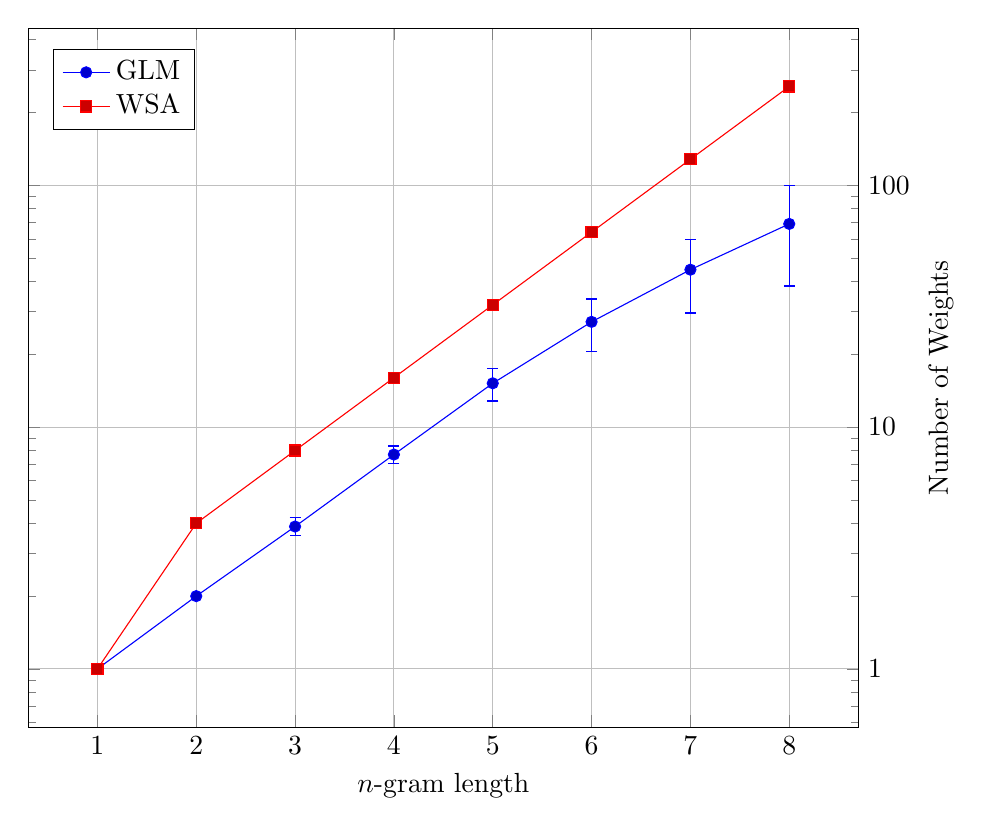
\begin{tikzpicture}[baseline]

\begin{axis}[
  xlabel = {$n$-gram length},
  xtick = {1, ..., 8},
  ylabel = {Number of Weights},
  yticklabel pos = right,
  ymode = log,
  minor y tick num = 4,
  log ticks with fixed point,
  grid = major,
  legend entries = {{GLM}, {WSA}},
  legend pos = north west,
  width = \textwidth,
]

% GLM
\addplot+[
  error bars/.cd,
  y dir = both,
  y explicit,
] table [y error = weights_error] {
  n  weights  weights_error
  1    1.00    0.00
  2    2.00    0.00
  3    3.88    0.33
  4    7.70    0.65
  5   15.17    2.35
  6   27.23    6.61
  7   44.74   15.12
  8   69.18   30.86
};

% WSA
\addplot+[
  error bars/.cd,
  y dir = both,
  y explicit,
] table [y error = weights_error] {
  n  weights  weights_error
  1    1.00  0.00
  2    4.00  0.00
  3    8.00  0.00
  4   16.00  0.00
  5   32.00  0.00
  6   64.00  0.00
  7  128.00  0.00
  8  256.00  0.00
};

\end{axis}

\end{tikzpicture}
\end{document}
